\documentclass{article}

\usepackage{amsmath, amssymb}
\usepackage{graphicx}

\title{Home Work 1}
\author{Author: Leul Shiferaw}

\begin{document}
	\maketitle
	
	\section{Task 1}
		\subsection{Deriving G(jw)}
		\noindent We start by representing the elements as in their Laplace Transform then apply voltage divider.\\
		\begin{align*}
			V_{out}&=V_{in}\frac{R}{\frac{1}{sC}+R}\\
				   &=V_{in}\frac{sRC}{1+sRC}\\
			G(s)&=\frac{V_{out}}{V_{in}}\\
			    &=\frac{sRC}{1+sRC}\\
			G(jw)&=\frac{jwRC}{1+jwRC}
		\end{align*}
		\subsection{Matlab Code}
			\subsubsection{True Plot}
			\begin{figure}[h!]
				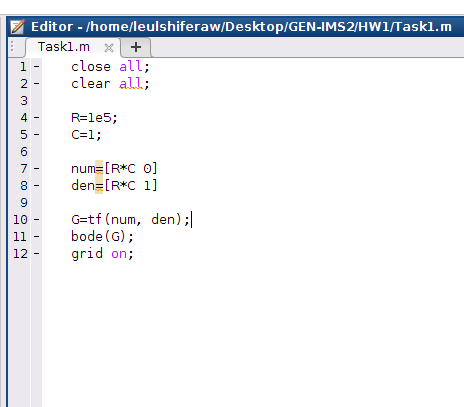
\includegraphics[width=10cm]{Task1_true.png}
				\caption{Code for true plot}
			\end{figure}
			\begin{figure}[h!]
				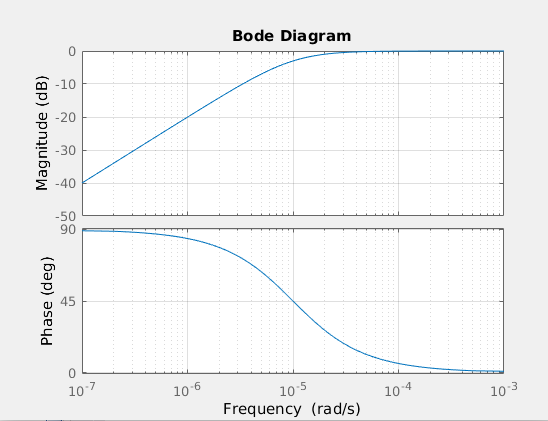
\includegraphics[width=10cm]{Task1_true_bode.png}
				\caption{Bode plot for true plot}
			\end{figure}
	\section{Task 2}
		\subsection{Deriving G(jw)}
		We start by representing the elements in their Laplace Transform and then applying voltage divider.\\
		\begin{align*}
			V_{out}&=V_{in}\frac{\frac{1}{sC}}{\frac{1}{sC}+R}\\
				&=V_{in}\frac{1}{1+sRC}\\
			G(s)&=\frac{V_{out}}{V_{in}}\\
				&=\frac{1}{1+sRC}\\
			G(jw)&=\frac{1}{1+jwRC}
		\end{align*}
	\newpage
		\subsection{Matlab Code}
			\subsubsection{True Plot}
			\begin{figure}[h!]
				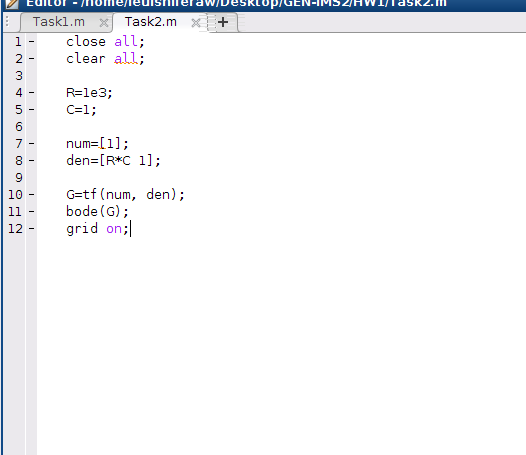
\includegraphics[width=10cm]{Task2_code.png}
				\caption{Code for bode plot}
			\end{figure}
			\begin{figure}[h!]
				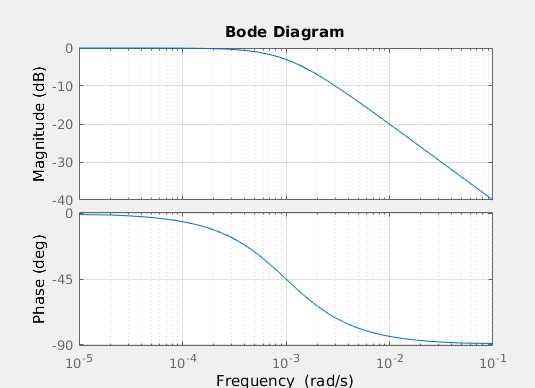
\includegraphics[width=10cm]{Task2_true.png}
				\caption{Bode plot}
			\end{figure}
	\newpage
	\section{Task 3}
		\subsection{Bode plots}
			\subsubsection{A}
			\begin{figure}[h!]
				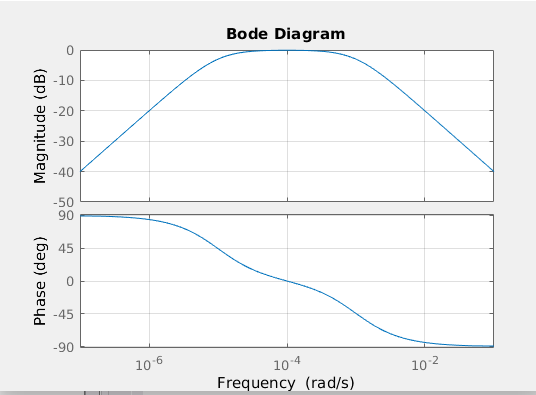
\includegraphics[width=5cm,height=5cm]{Task3_A.png}
				\caption{Bode plot for Task 3 a}
			\end{figure}
			\begin{figure}[h!]
				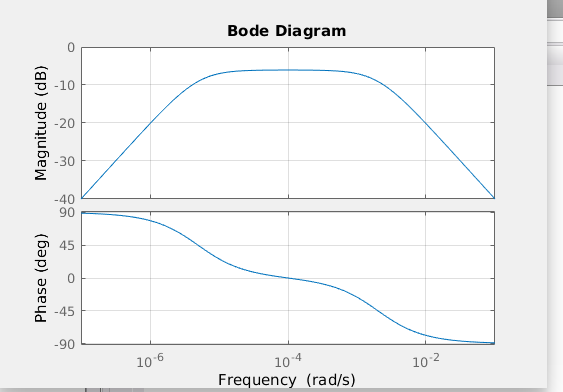
\includegraphics[width=10cm]{Task3_B.png}
				\caption{Bode plot Task 3 b}
			\end{figure}
			\begin{figure}[h!]
				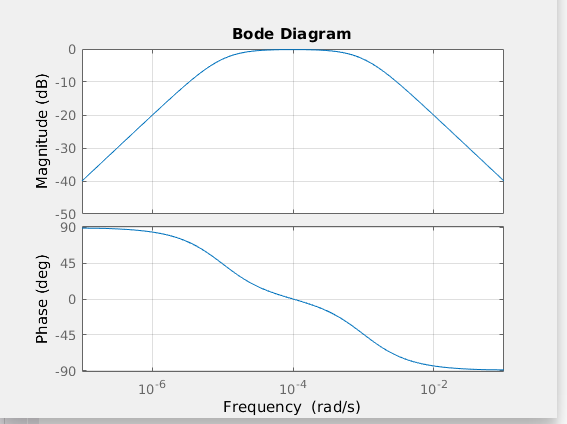
\includegraphics[width=10cm]{Task3_C.png}
				\caption{Bode plot Task 3 c}
			\end{figure}
		
\end{document}